\documentclass{article}

\usepackage[utf8]{inputenc}
\usepackage{graphicx}
\usepackage{silence}

\WarningFilter{latex}{Text page}

\makeatletter
\setlength{\@fptop}{0pt}
\setlength{\@fpbot}{0pt plus 1fil}
\makeatother

% \title{Molecular Dynamics Benchmark for Leadership-Class HPC Machines}
% \author{Andre Merzky, Manuel O. Maldonado, Matteo Turilli, Shantenu Jha}
% \date{December 2017}

\begin{document}

% \maketitle

% \noindent Workload and Machines:
% \begin{itemize}
% 	\item Physical system: \ldots; n atoms.
% 	\item Executable: GROMACS OpenMPI.
% 	\item Emulator: Synapse.
% 	\item Number of tasks: 32--16384.
% 	\item Number of cores per task: 32.
% 	\item Number of nodes on Titan: 2--16384.
% 	\item Machine: Titan.
% \end{itemize}

\begin{figure}
  \centering
  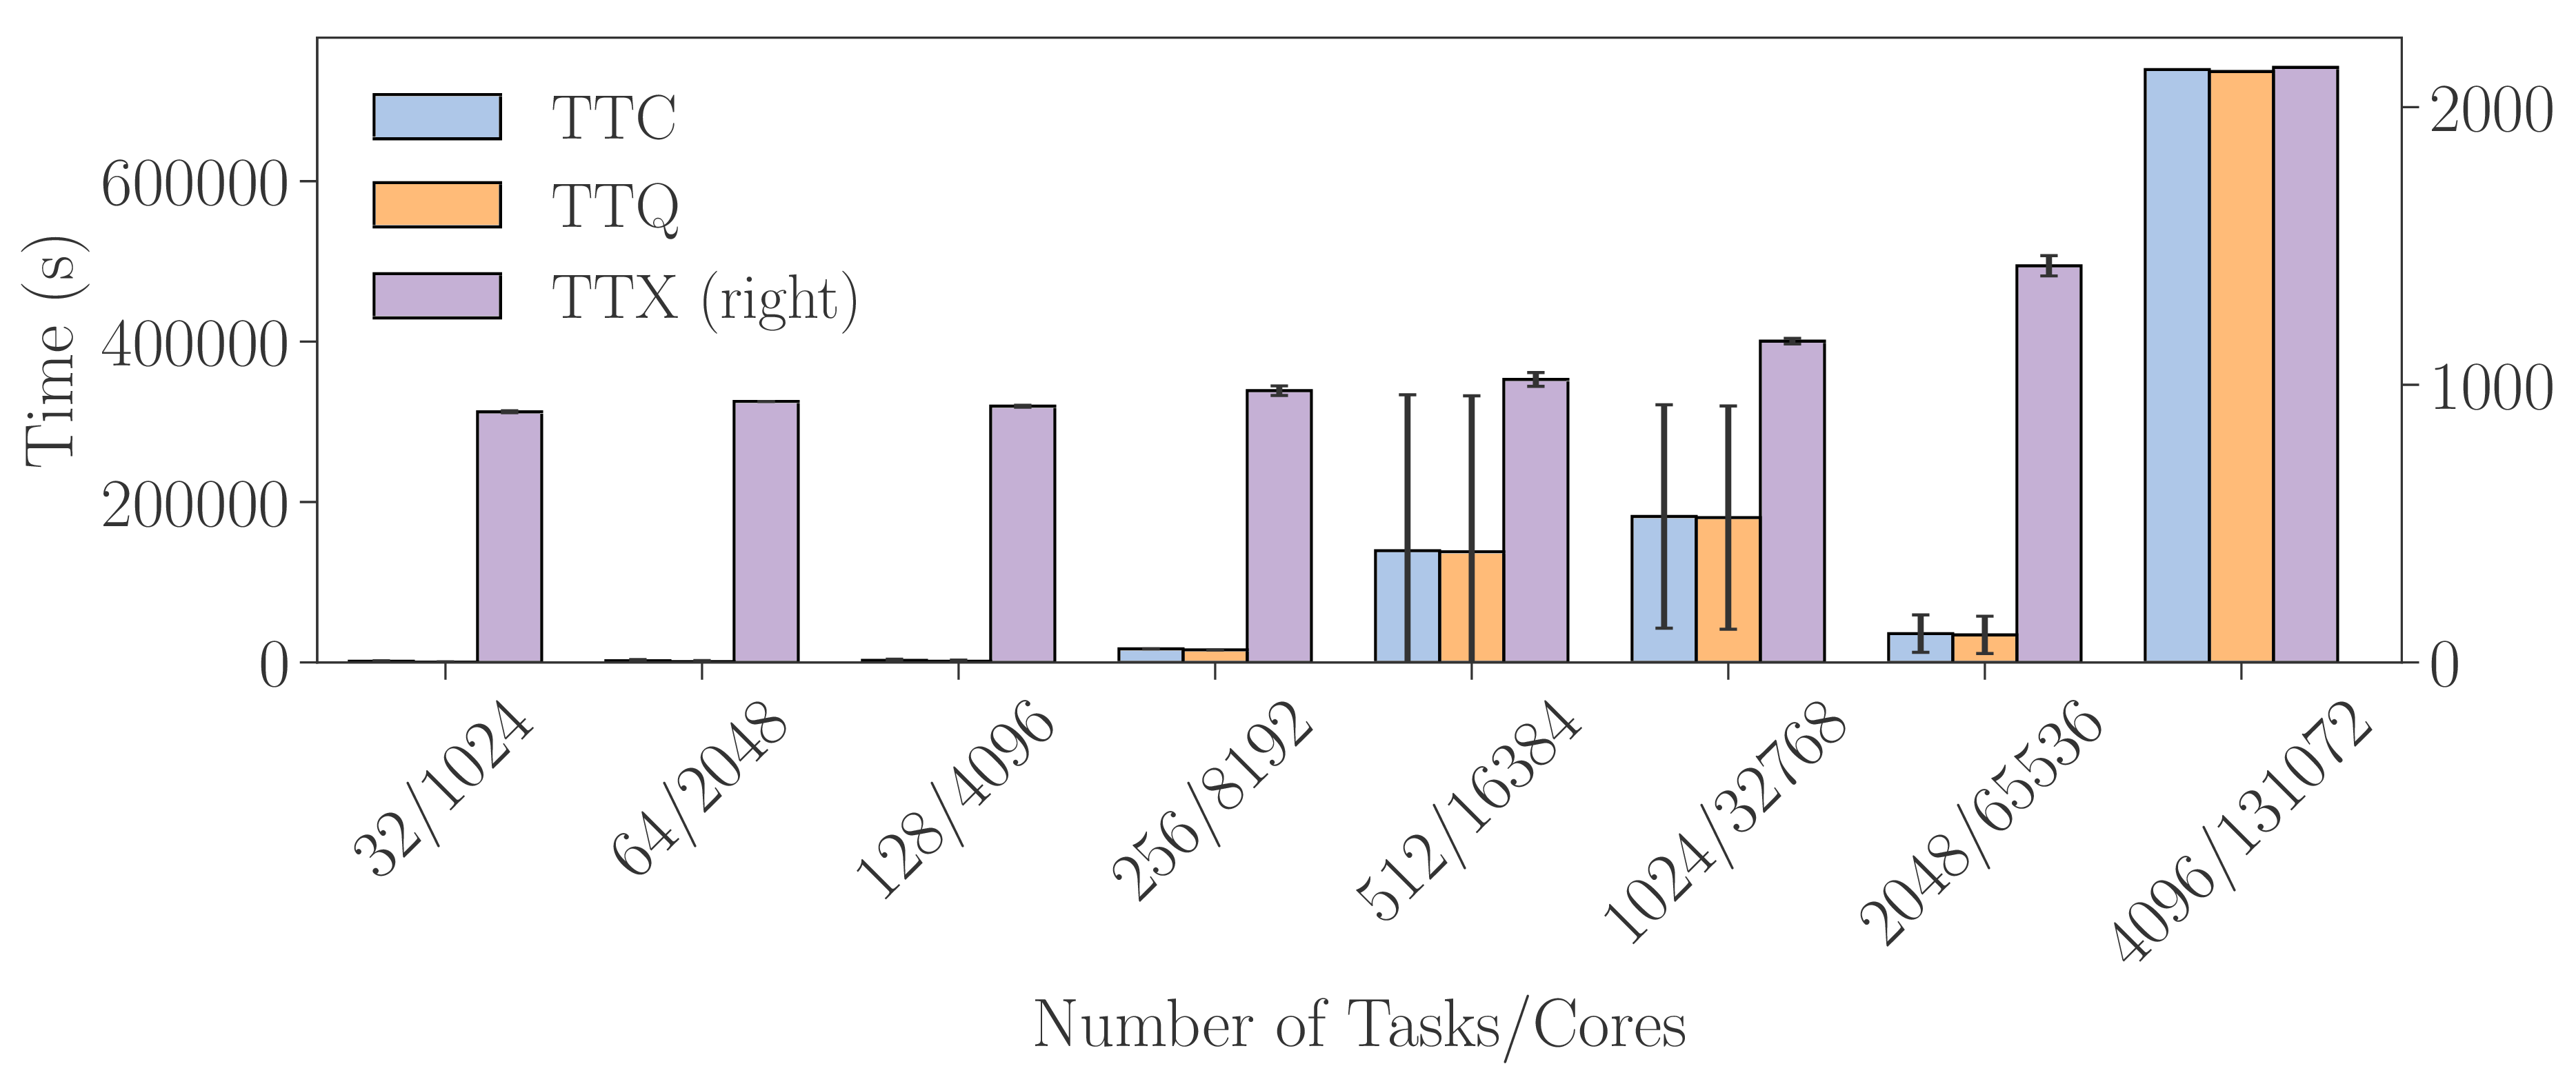
\includegraphics[width=\columnwidth]{figures/screen_titan_rp_synapse_weak_scaling.png}
  \caption{\textbf{Weak scaling:} For the given workload, RADICAL-Pilot
	weak scales linearly between 64 and 1024 nodes; sublinearly between 1024
	and 8192 nodes. Runs with 16384 nodes fail for bugs in the current
	implementation of OpenMPI. }\label{fig:ws-ttc}
\end{figure}

\begin{figure}
  \centering
  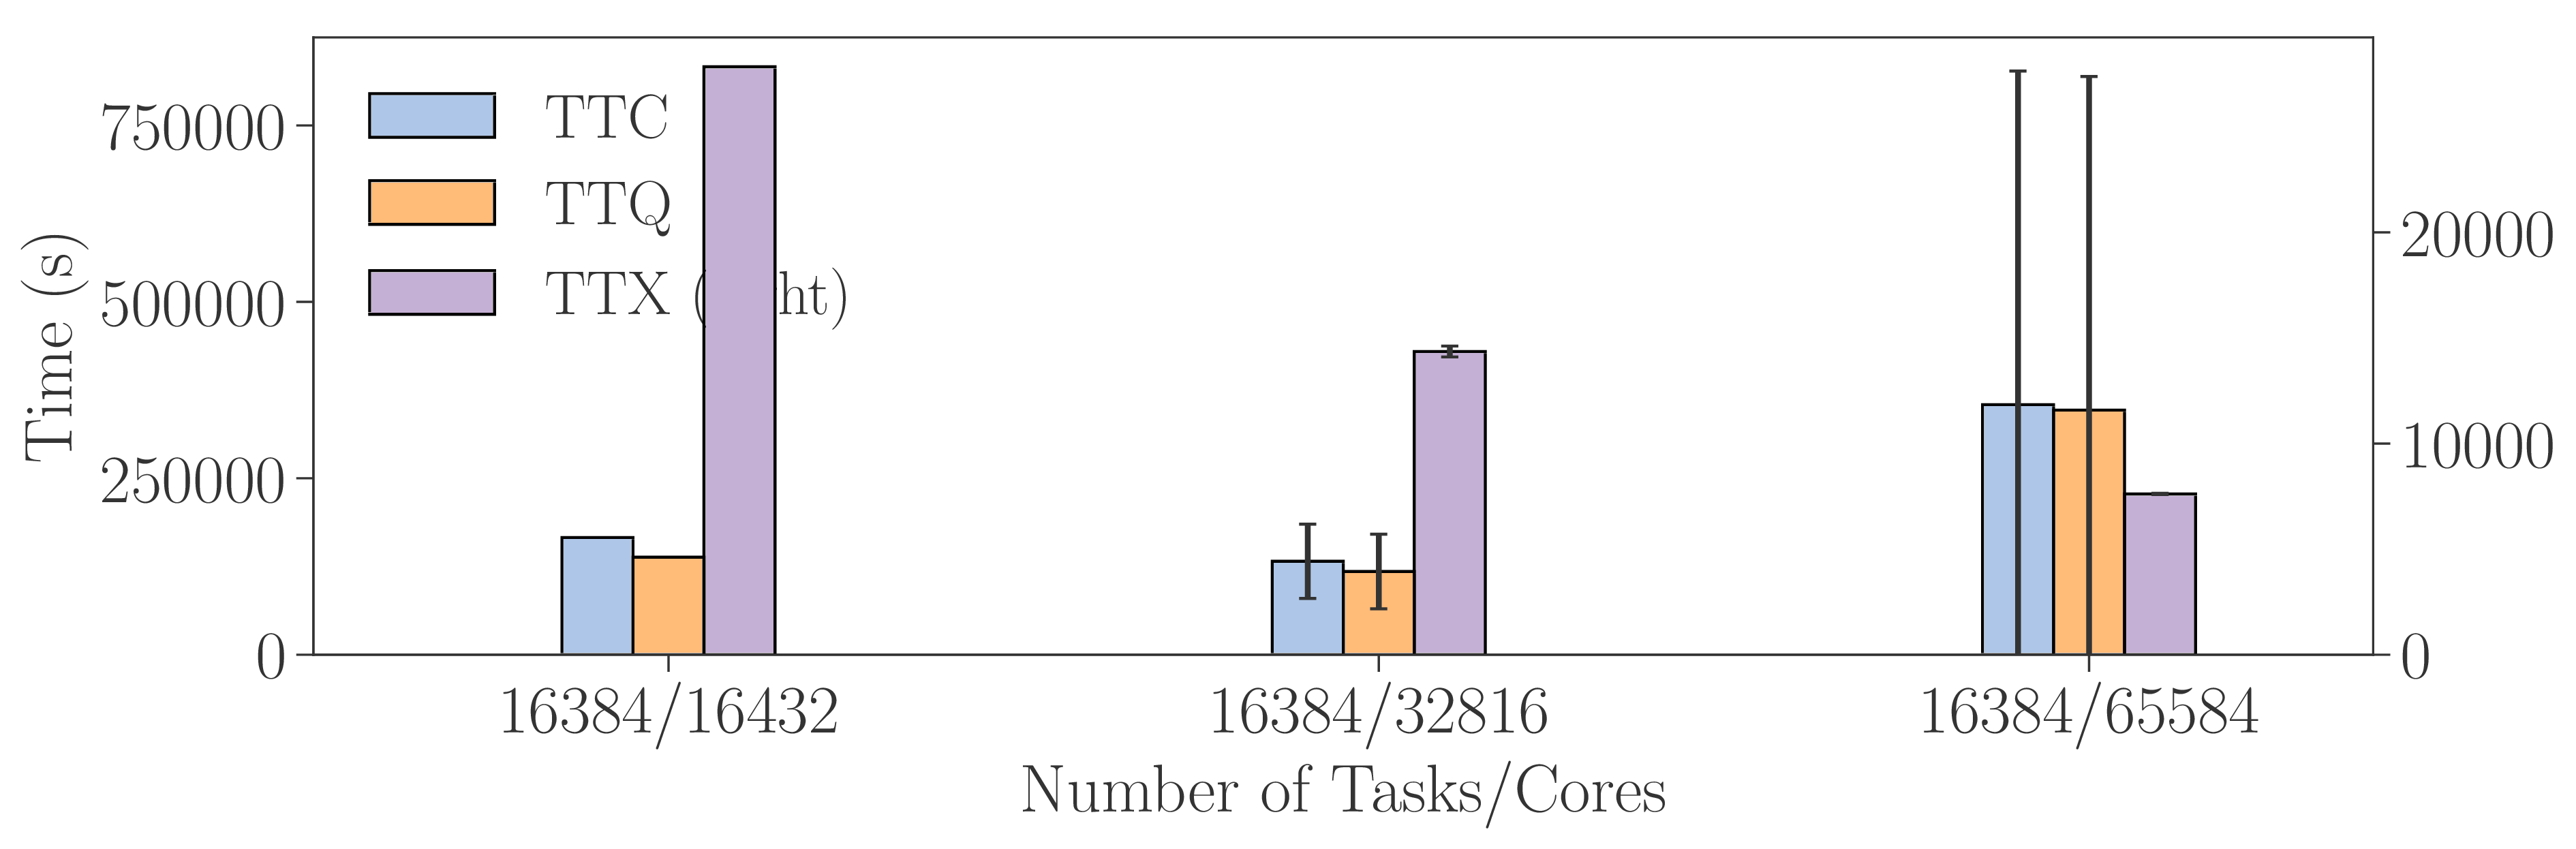
\includegraphics[width=\columnwidth]{figures/screen_titan_rp_synapse_strong_scaling.png}
  \caption{\textbf{Strong scaling:} For the given workload with 16384 tasks,
	RADICAL-Pilot strong scales linearly between 1024 and 4096 nodes. Runs
	with more than 8192 fail for bugs in the current implementation of
	OpenMPI.}\label{fig:ss-ttc}
\end{figure}

\begin{figure}
  \centering
  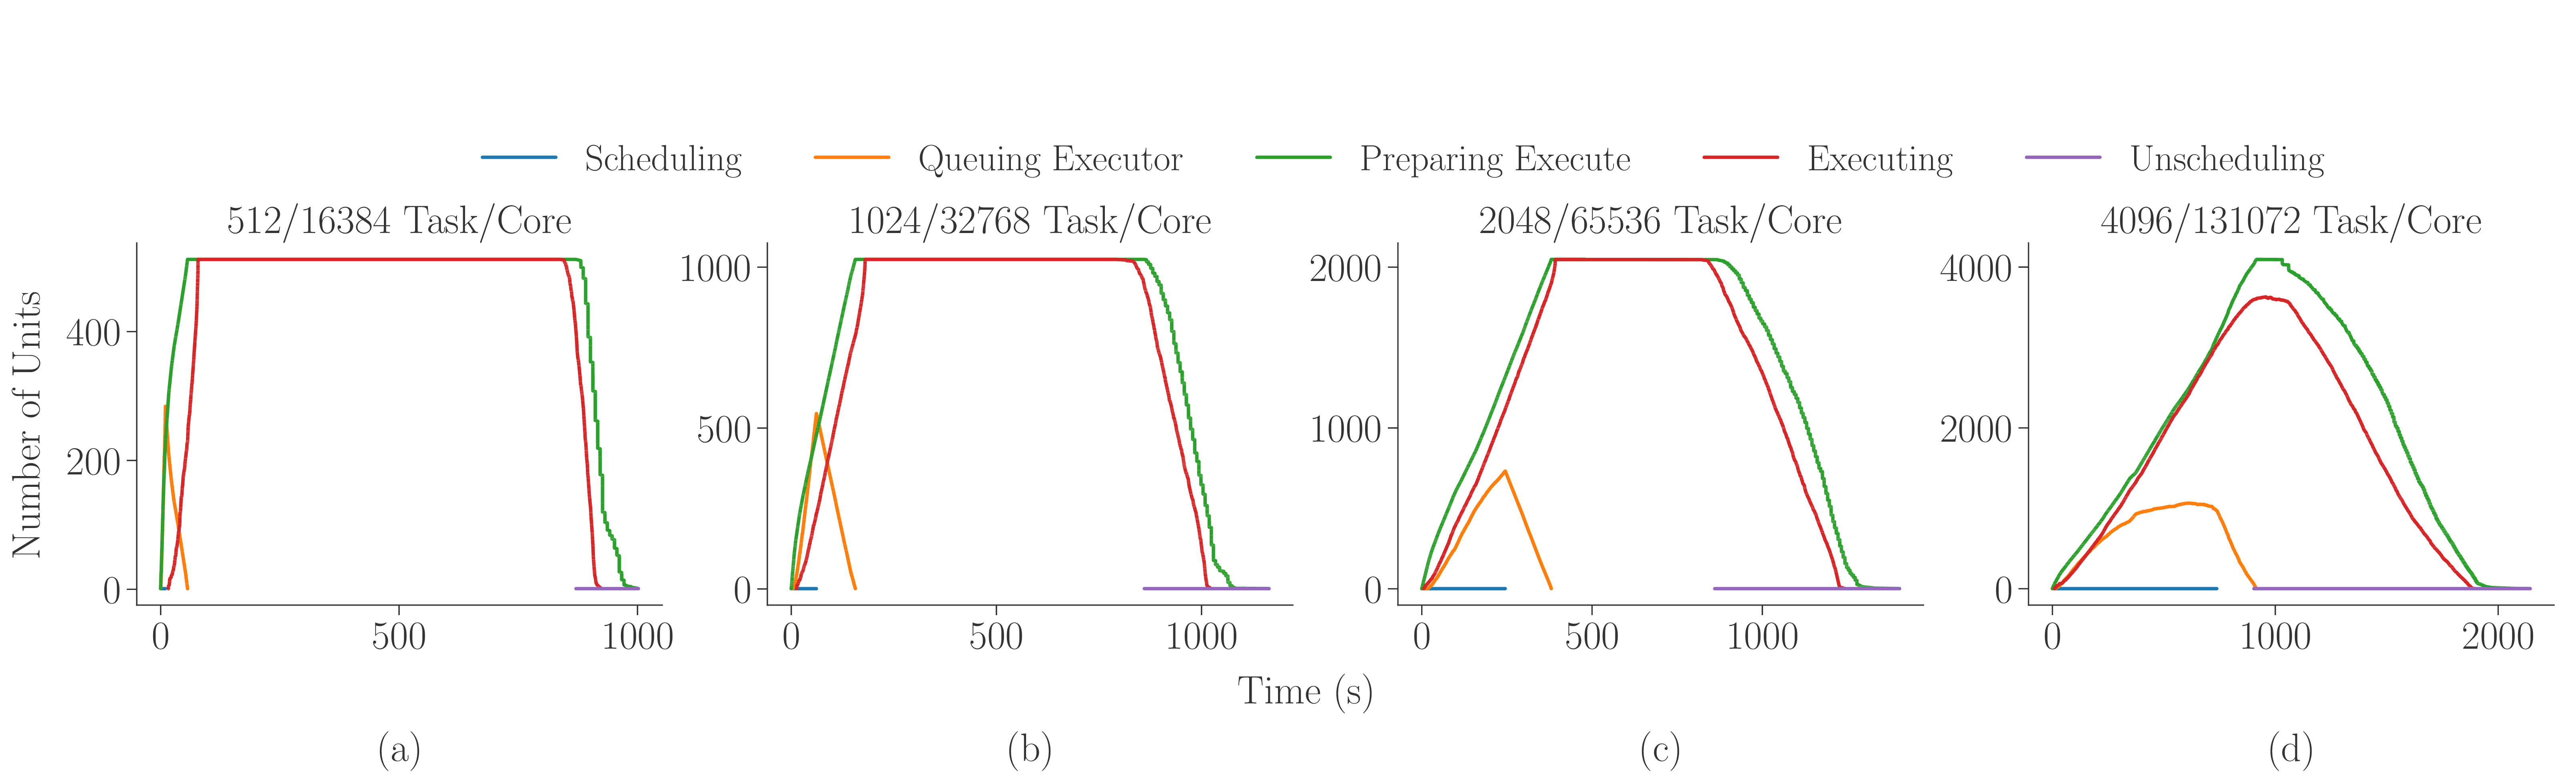
\includegraphics[width=\textwidth]{figures/screen_titan_rp_synapse_weak_scaling_concurrency_horizontal.png}
  \caption{\textbf{Concurrency of weak scaling:} Sublinear weak scaling
  performance depends from a decreased concurrency of the workload execution.
  RADICAL-Pilot is not able to use all the available cores, resulting in
  fewer tasks executing at the same time.}\label{fig:ws-concurrency}
\end{figure}

\begin{figure}
  \centering
  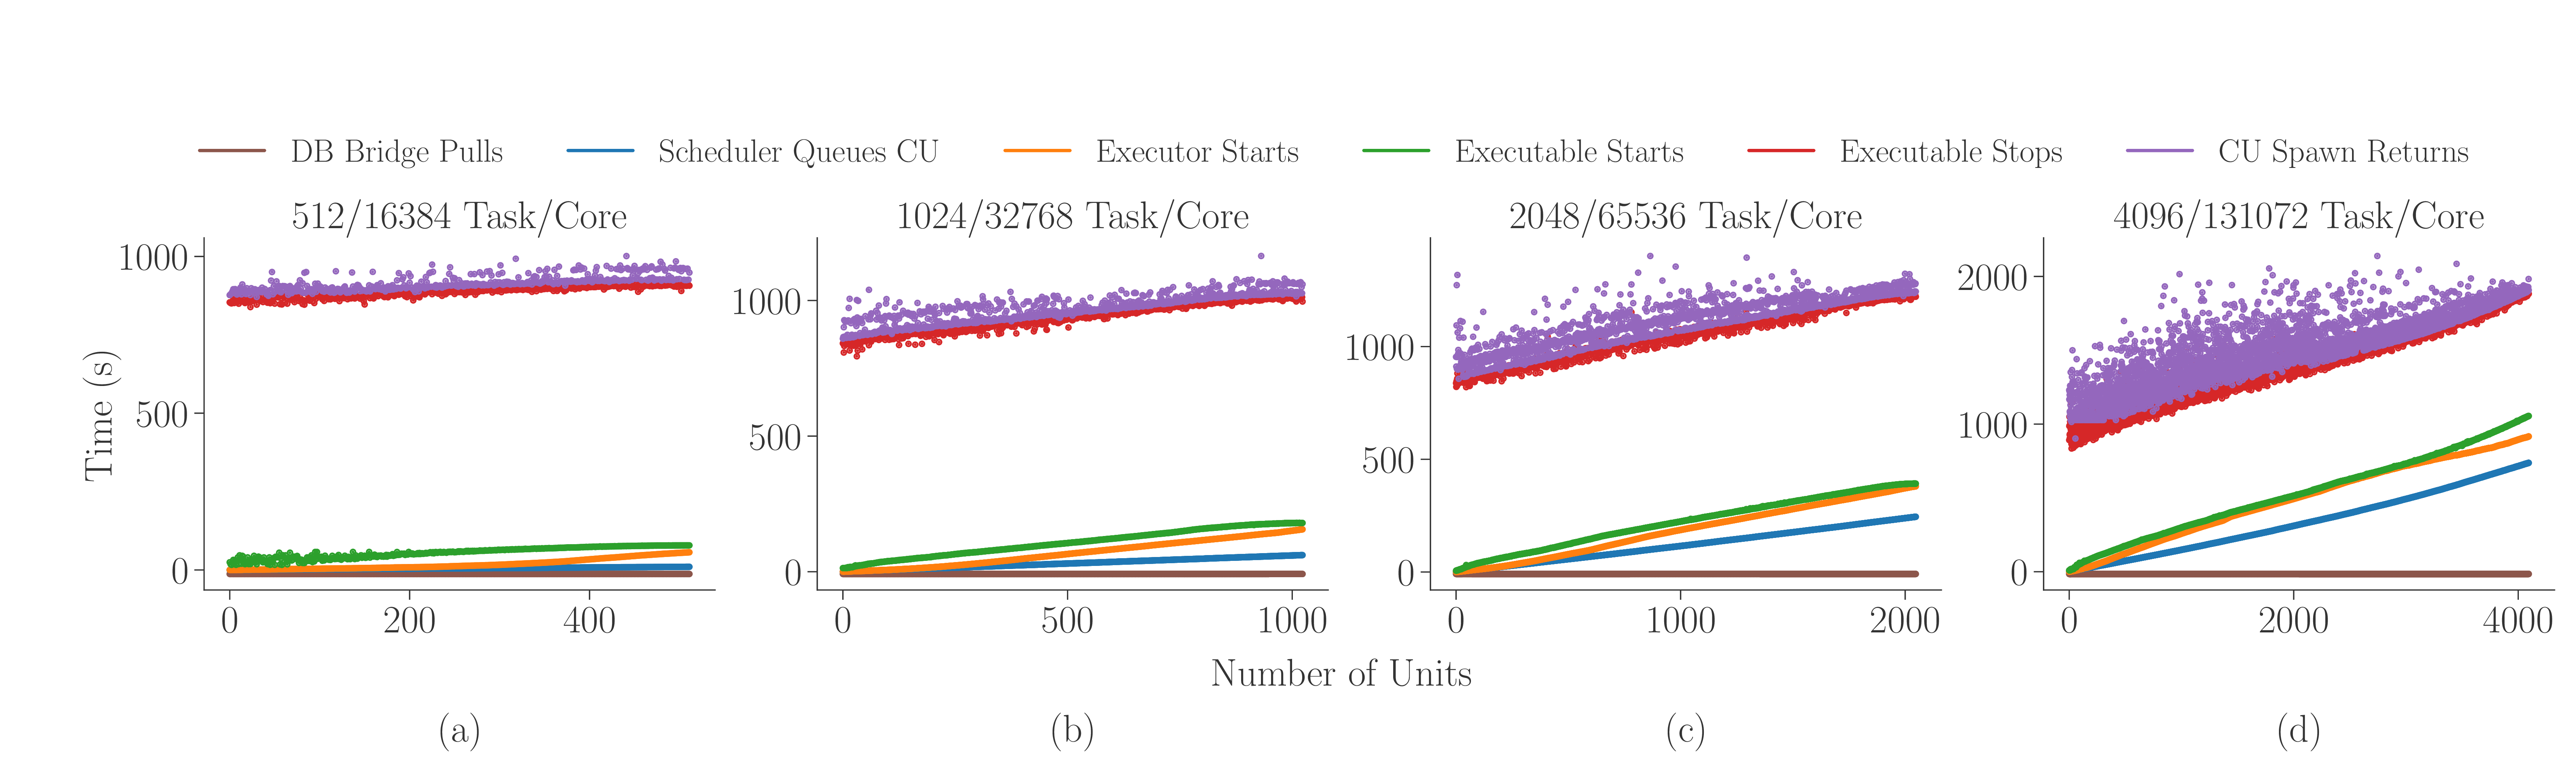
\includegraphics[width=\textwidth]{figures/screen_titan_rp_synapse_weak_scaling_events_timeline_horizontal.png}
  \caption{\textbf{Relevant events of weak scaling profiling:} Sublinear weak
	scaling depends on the current implementation of the Scheduler component
	and, to a lesser measure, of the Executor components of RADICAL-Pilot.
	Both components are part of RADICAL-Pilot Agent, the software executed on
	the resource compute nodes. }\label{fig:ws-events}
\end{figure}

\begin{figure}
  \centering
  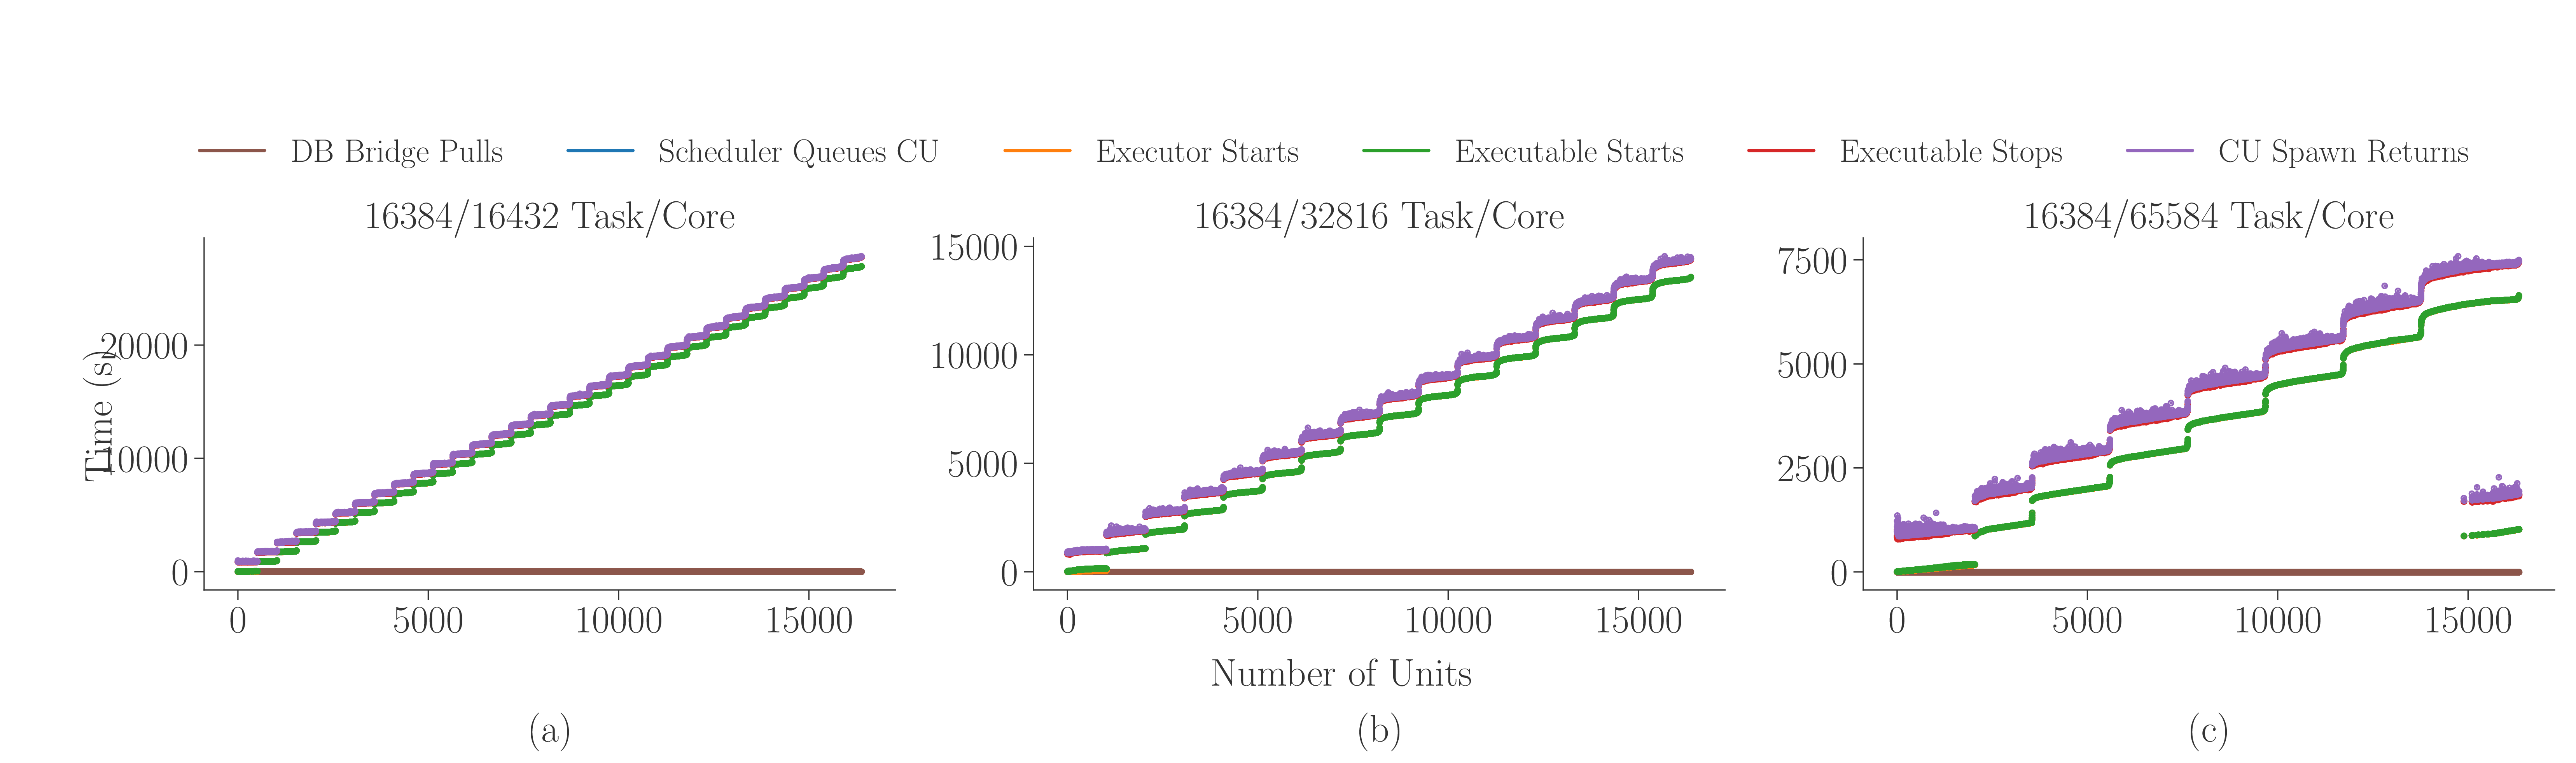
\includegraphics[width=\textwidth]{figures/screen_titan_rp_synapse_strong_scaling_events_timeline_horizontal.png}
  \caption{\textbf{Relevant events of strong scaling profiling:}
  RADICAL-Pilot sequentially executes sets of units. The performance of the
  execution of each set slightly decreases with the increasing of the number
  of cores. The loss of performance produces a marginal deviation from linear
  strong scaling.}\label{fig:ss-events}
\end{figure}

\begin{figure}
  \centering
  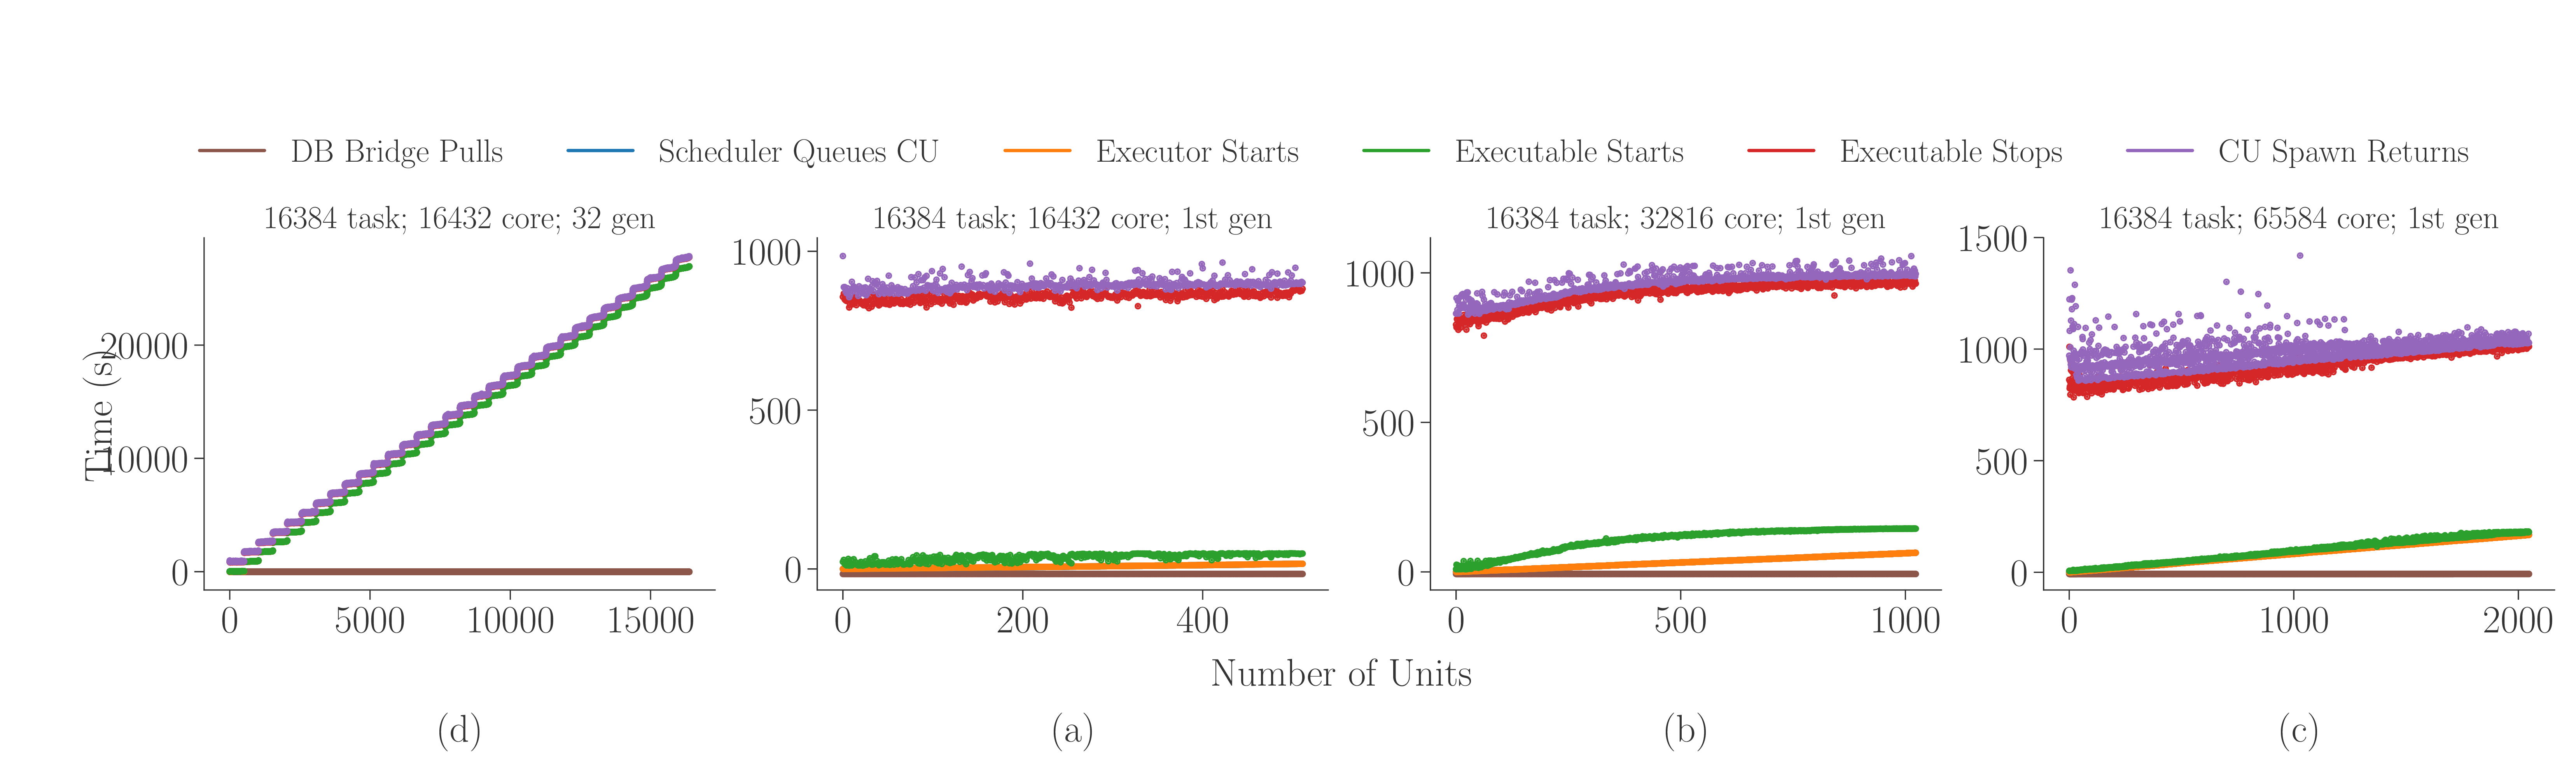
\includegraphics[width=\textwidth]{figures/screen_titan_rp_synapse_strong_scaling_events_timeline_1stgen_horizontal.png}
  \caption{\textbf{Performance of the Scheduler component in strong scaling:}
	The performance of the Scheduler component depends on the size of the
	pilot, i.e., on the number of compute nodes/cores used to schedule the
	tasks of the workload. The Scheduler performance is instead invariant to
	the number of the tasks scheduled. }\label{fig:ss-events-1stgen}
\end{figure}

\end{document}